\section{Transição de estados}

Sendo o vetor de estados do robô dado por \eqref{eq:x}, e o vetor de entradas por \eqref{eq:u}, têm-se que a odometria, dado pelo modelo dinâmico incremental do sistema é dada por \eqref{eq:f}.

\begin{equation}\label{eq:x}
	\+x_t = \begin{bmatrix}
		x_t & y_t & zt
	\end{bmatrix}^T
\end{equation}


\begin{equation}\label{eq:u}
	\+u_t = \begin{bmatrix}
		\Delta s_l & \Delta s_r
	\end{bmatrix}^T
\end{equation}

\begin{equation}\label{eq:f}
	\widehat{\+x}_t = \+f(\+x_{t-1},\+u_t) = \+x_{t-1} + \begin{bmatrix}
		 \dfrac{\Delta s_r + \Delta s_l}{2}\cos\left(\theta_{t-1} + \dfrac{\Delta s_r - \Delta s_l}{2\cdot l}  \right) \\[2ex]
		 \dfrac{\Delta s_r + \Delta s_l}{2}\sin\left(\theta_{t-1} + \dfrac{\Delta s_r - \Delta s_l}{2\cdot l}  \right) \\[2ex]
		  \dfrac{\Delta s_r - \Delta s_l}{l}
	\end{bmatrix}
\end{equation}

Realizando a derivada parcial da odometria em relação aos estados do sistema, obtém-se o jacobiano em relação aos estados, dado por \eqref{eq:Fx}. Fazendo o mesmo processo em relação ao vetor de entradas, obtém-se o jacobiano a associado às entradas, \eqref{eq:Fu}, com as derivadas parciais listadas de \eqref{eq:fxsl} à \eqref{eq:fzsr}.

\begin{equation}\label{eq:Fx}
\begin{split}
	\+{F_x} &= \begin{bmatrix}
	\dfrac{\partial \+f}{\partial x} & 
	\dfrac{\partial \+f}{\partial y} &
	\dfrac{\partial \+f}{\partial z}
\end{bmatrix} = \begin{bmatrix}
	\dfrac{\partial f_x}{\partial  x } & 	\dfrac{\partial f_x}{\partial y}  & 	\dfrac{\partial f_x}{\partial z} \\[2ex]
	\dfrac{\partial f_y}{\partial  x } & 	\dfrac{\partial f_y}{\partial y}  & 	\dfrac{\partial f_y}{\partial z} \\[2ex]
	\dfrac{\partial f_z}{\partial  x } & 	\dfrac{\partial f_z}{\partial y}  & 	\dfrac{\partial f_z}{\partial z} 
\end{bmatrix} \\
&=\begin{bmatrix}
	1 & 0  & \dfrac{\Delta s_r + \Delta s_l}{2}\sin\left( \theta_{t-1} + \dfrac{\Delta s_r - \Delta s_l}{2\cdot l} \right)  \\[2ex]
	0 & 1  & 	 \dfrac{\Delta s_r + \Delta s_l}{2}\cos\left( \theta_{t-1} + \dfrac{\Delta s_r - \Delta s_l}{2\cdot l} \right)  \\[2ex]
	0 & 0  & 1
\end{bmatrix}
\end{split}
\end{equation}



\begin{equation}\label{eq:Fu}
	\+{F_u} = \begin{bmatrix}
		\dfrac{\partial \+f}{\partial \Delta s_l} & 
		\dfrac{\partial \+f}{\partial \Delta s_r}
	\end{bmatrix} = \begin{bmatrix}
	\dfrac{\partial f_x}{\partial \Delta s_l } & 	\dfrac{\partial f_x}{\partial \Delta s_r } \\[2ex]
	\dfrac{\partial f_y}{\partial \Delta s_l } & 	\dfrac{\partial f_y}{\partial \Delta s_r } \\[2ex]
	\dfrac{\partial f_z}{\partial \Delta s_l } & 	\dfrac{\partial f_z}{\partial \Delta s_r }
	\end{bmatrix}
\end{equation}

\begin{equation}\label{eq:fxsl}
	\dfrac{\partial f_x}{\partial \Delta s_l } =  
	\dfrac{1}{2}\cos\left( \theta_{t-1} + \dfrac{\Delta s_r - \Delta s_l}{2\cdot l}\right)  + \dfrac{\Delta s_r + \Delta s_l}{2\cdot2 \cdot l}\sin\left( \theta_{t-1} + \dfrac{\Delta s_r - \Delta s_l}{2\cdot l}\right) 
\end{equation}

\begin{equation}\label{eq:fxsr}
\dfrac{\partial f_x}{\partial \Delta s_r } =  
\dfrac{1}{2}\cos\left( \theta_{t-1} + \dfrac{\Delta s_r - \Delta s_l}{2\cdot l}\right)  - \dfrac{\Delta s_r + \Delta s_l}{2\cdot2 \cdot l}\sin\left( \theta_{t-1} + \dfrac{\Delta s_r - \Delta s_l}{2\cdot l}\right) 
\end{equation}

\begin{equation}\label{eq:fysl}
\dfrac{\partial f_y}{\partial \Delta s_l } =  
\dfrac{1}{2}\sin\left( \theta_{t-1} + \dfrac{\Delta s_r - \Delta s_l}{2\cdot l}\right)  - \dfrac{\Delta s_r + \Delta s_l}{2\cdot2 \cdot l}\cos\left( \theta_{t-1} + \dfrac{\Delta s_r - \Delta s_l}{2\cdot l}\right) 
\end{equation}

\begin{equation}\label{eq:fysr}
\dfrac{\partial f_y}{\partial \Delta s_r } =  
\dfrac{1}{2}\sin\left( \theta_{t-1} + \dfrac{\Delta s_r - \Delta s_l}{2\cdot l}\right)  + \dfrac{\Delta s_r + \Delta s_l}{2\cdot2 \cdot l}\cos\left( \theta_{t-1} + \dfrac{\Delta s_r - \Delta s_l}{2\cdot l}\right) 
\end{equation}

\begin{equation}\label{eq:fzsl}
\dfrac{\partial f_y}{\partial \Delta s_l } = -\dfrac{1}{l}
\end{equation}

\begin{equation}\label{eq:fzsr}
\dfrac{\partial f_y}{\partial \Delta s_r } = \dfrac{1}{l}
\end{equation}

Aplicando a odometria pelo modelo incremental, observa-se na \autoref{fig:odometry_raw} que rapidamente a posição obtida por meio da integração dos estados diverge da posição real, sendo uma informação que não confiável, sendo necessário a fusão da mesma com outros sensores para a obtenção de uma localização precisa.

\begin{figure}[H]
	\centering
	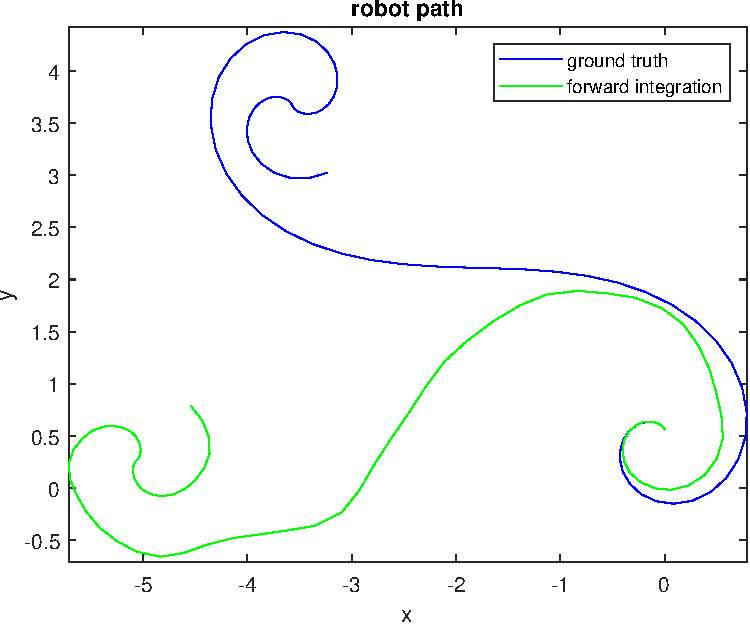
\includegraphics[width=0.75\linewidth]{img/odometry_raw}
	\caption{Caminho percorrido pelo robô $\times$ odometria obtida pela integração do  modelo cinemático incremental direto.}
	\label{fig:odometry_raw}
\end{figure}

\clearpage

A implementação da função de transição dos estados é dada abaixo:

\begin{lstlisting}[language=Octave]
function [f, F_x, F_u] = transitionFunction(x,u, l)
% [f, F_x, F_u] = transitionFunction(x,u,l) predicts the state x at time t given
% the state at time t-1 and the input u at time t. F_x denotes the Jacobian
% of the state transition function with respect to the state evaluated at
% the state and input provided. F_u denotes the Jacobian of the state
% transition function with respect to the input evaluated at the state and
% input provided.
% State and input are defined according to "Introduction to Autonomous Mobile Robots", pp. 337

%STARTRM

f = x +  [(u(1) + u(2))/2*cos(x(3) + ((u(2)-u(1))/(2*l))); ...
(u(1) + u(2))/2*sin(x(3) + ((u(2)-u(1))/(2*l))); ...
(u(2) - u(1))/l ];

F_x = [1, 0, -(u(1) + u(2))/2*sin(x(3)+(u(2)-u(1))/(2*l)); ...
0, 1, (u(1) + u(2))/2*cos(x(3)+(u(2)-u(1))/(2*l)); ...
0, 0, 1];

F_u = [(cos(x(3) + (u(2)-u(1))/(2*l))/2 + (u(1) + u(2))/(2*2*l)*sin(x(3) + (u(2)-u(1))/(2*l))), ...
(cos(x(3) + (u(2)-u(1))/(2*l))/2 - (u(1) + u(2))/(2*2*l)*sin(x(3) + (u(2)-u(1))/(2*l))); ...
(sin(x(3) + (u(2)-u(1))/(2*l))/2 - (u(1) + u(2))/(2*2*l)*cos(x(3) + (u(2)-u(1))/(2*l))), ...
(sin(x(3) + (u(2)-u(1))/(2*l))/2 + (u(1) + u(2))/(2*2*l)*cos(x(3) + (u(2)-u(1))/(2*l))); ...
-1/l, 1/l];    


%ENDRM

\end{lstlisting}



\clearpage

\section{Atualização do estado}

\subsection{Função de medição}

Dada a refência de uma linha dada pelo mapa, pelo vetor $\begin{bmatrix} \alpha_t^j & r_t^j \end{bmatrix}^T$, no referencial inercial do mundo, porém, para utilizar esses dados, é preciso saber qual a posição das linhas em relação ao robô, pois assim o mapa estará no mesmo referencial dos sensores que serão utilizados na percepção. Com isso, realiza-se a transformação para o referencial do robô no estado atual por meio de \eqref{eq:h}. O jacobiano dessa transformação pode ser obtido aplicando as derivadas parciais em relação aos estados, como feito em \eqref{eq:H}.

\begin{equation}\label{eq:h}
	\+h(\widehat{\+x}_t,\+m^j) = \begin{bmatrix}
		\alpha_t^j - \widehat{\theta}_t \\
		r_t^j - \widehat{x}_t\cos(\alpha_t^j) - \widehat{y}_t\sin(\alpha_t^j)
	\end{bmatrix}
\end{equation}

\begin{equation}\label{eq:H}
	\+H^J = \begin{bmatrix}
		\dfrac{\partial \alpha_t^j}{\partial \widehat{x}} & \dfrac{\partial \alpha_t^j}{\partial \widehat{y}} & \dfrac{\partial \alpha_t^j}{\partial \widehat{z}} \\[2ex]
		\dfrac{\partial r_t^j}{\partial \widehat{x}} & \dfrac{\partial r_t^j}{\partial \widehat{y}} & \dfrac{\partial r_t^j}{\partial \widehat{z}}
	\end{bmatrix} = \begin{bmatrix}
		0 & 0 & -1 \\
		-\cos(\alpha_t^j) & -\sin(\alpha_t^j) & 0
	\end{bmatrix}
\end{equation}

A implementação da função de medição é dada abaixo:

\begin{lstlisting}[language=Octave]
function [h, H_x] = measurementFunction(x, m)
% [h, H_x] = measurementFunction(x, m) returns the predicted measurement
% given a state x and a single map entry m. H_x denotes the Jacobian of the
% measurement function with respect to the state evaluated at the state
% provided.
% Map entry and state are defined according to "Introduction to Autonomous Mobile Robots" pp. 337

%STARTRM
h = [m(1) - x(3);
m(2) - x(1)*cos(m(1)) - x(2)*sin(m(1))];

H_x = [0, 0, -1;
-cos(m(1)), -sin(m(1)), 0];

%ENDRM

[h(1), h(2), isRNegated] = normalizeLineParameters(h(1), h(2));

if isRNegated 
H_x(2, :) = - H_x(2, :);
end
\end{lstlisting}

\clearpage


\subsection{Filtro}

Para aplicação da correção utilizando filtro de Kalman estendido, é necessário inicialmente realizar a etapa de predição, feita anteriormente pela função de transição de estados. Além disso, é preciso saber a covariância do erro \textit{a priori} ($\widehat{\+P}_t$), que é obtida com base na matriz de covariância $\+Q$, dada por \eqref{eq:Q}.

\begin{equation}\label{eq:Q}
	\+Q = \begin{bmatrix}
		k|\Delta s_r| & 0 \\
		0 & k|\Delta s_l|
	\end{bmatrix}
\end{equation}

Sendo assim, a covariância do erro \textit{a priori} é dada por \eqref{eq:Ppriori}, utilizando os jacobianos obtidos em \eqref{eq:Fx} e \eqref{eq:Fu}.

\begin{equation}\label{eq:Ppriori}
	\widehat{\+P}_t = \+{F_x}\+P\+{F_x}^T + \+{F_u}\+Q\+{F_u}^T 
\end{equation}

Realizada a predição, é feita a etapa de correção, onde uma vez feito o \textit{matching} do estado predito com a leitura dos sensores exteroceptivos, é obtida a inovação ($\+S$), que permite a obtenção do ganho de Kalman ($\+K$) que é utilizado para realização da correção propriamente dita.

Em \eqref{eq:S} é obtida a inovação com base na covariância da predição e o jacobiano do sensor, obtido em \eqref{eq:H}, além da matriz de covariância do sensor $\+R$. Por fim, o ganho de Kalman é conforme \eqref{eq:K}, e a correção é feita em \eqref{eq:correcao}, obtendo a predição \textit{a posteriori}.

\begin{equation}\label{eq:S}
	\+S_t = \+H\widehat{\+P}_t\+H^T + \+R_t
\end{equation}

\begin{equation}\label{eq:K}
	\+K_t = \widehat{\+P}_t\+H^T\+S^{-1}
\end{equation}

\begin{equation}\label{eq:correcao}
	\widehat{\+x}_{t|t} = 	\widehat{\+x}_{t|t-1} + \+K_t \widetilde{\+y}_t
\end{equation}

Por meio da filtragem da odometria utilizando filtro de Kalman extendido, fundindo os dados juntamente à medida da percepção do robô, observa-se na \autoref{fig:odometry_filtered} que a localização do robô se torna precisa, acompanhando a trajetória do mesmo com fidelidade.


\begin{figure}[H]
	\centering
	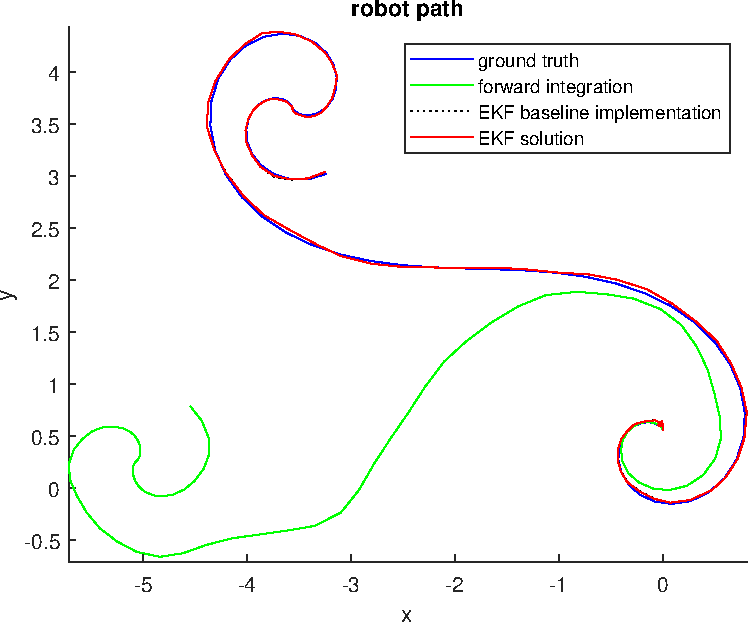
\includegraphics[width=0.75\linewidth]{img/odometry_filtered}
	\caption{Correção da odometria por meio do filtro de Kalman extendido.}
	\label{fig:odometry_filtered}
\end{figure}

\begin{lstlisting}[language=Octave]
function [x_posteriori, P_posteriori] = filterStep(x,P,u,Z,R,M,k,g,l)
Q = [k*abs(u(2)) 0; 0 k*abs(u(1))]; 

[x_priori, F_x, F_u] = transitionFunction(x, u, l); 
P_priori = F_x*P*F_x' + F_u*Q*F_u';

if size(Z,2) == 0
x_posteriori = x_priori;
P_posteriori = P_priori;
return;
end

[v, H, R] = associateMeasurements(x_priori, P_priori, Z, R, M, g);

y = reshape(v, [], 1);
H = reshape(permute(H, [1,3,2]), [], 3);
R = blockDiagonal(R);

S = H*P_priori*H'+R; %S is the innovation covariance matrix
K = P_priori*H'/S;

x_posteriori = x_priori + K * y;
P_posteriori = (eye(size(P_priori)) - K*H) * P_priori;
\end{lstlisting}

\clearpage

\section{Experimento V-REP}

Ao executar a simulação de localização incremental no CoppeliaSim, utilizando a fusão dos dados de odometria com os dados obtidos com o LiDAR comparados ao mapa, obtém-se uma localização precisa, como visto na \autoref{fig:vrep}, onde o robô \textit{ghost} está posicionado de forma coincidente ao robô real. Na \autoref{fig:measuement}, observba-se o \textit{match} feito entre as retas presentes no mapa, transformadas para o referencial do robô, e as retas obtidas por meio da percepção. Mesmo com o casamento de apenas algumas retas, a correção da localização é poderosa.

\begin{figure}[H]
	\centering
	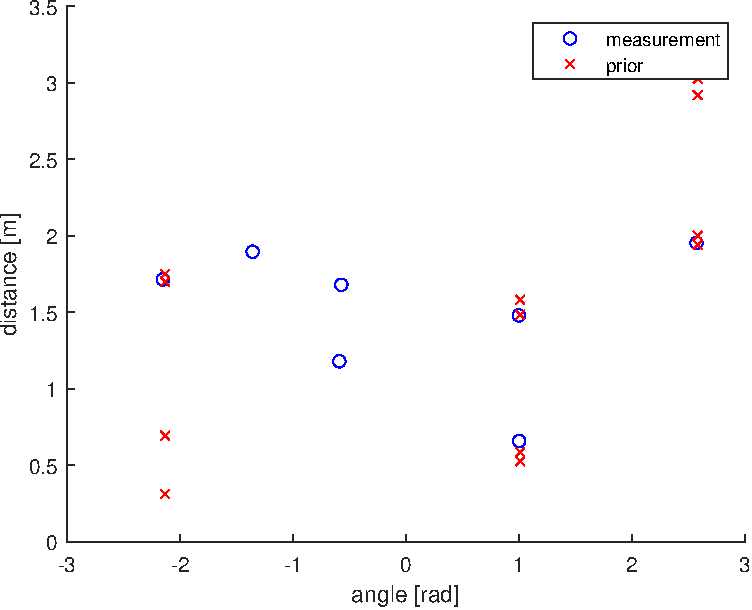
\includegraphics[width=0.65\linewidth]{img/measuement}
	\caption{Representação das retas do mapa (prior) e as retas obtidas pelo LiDAR no espaço de Hough.}
	\label{fig:measuement}
\end{figure}

\begin{figure}[H]
	\centering
	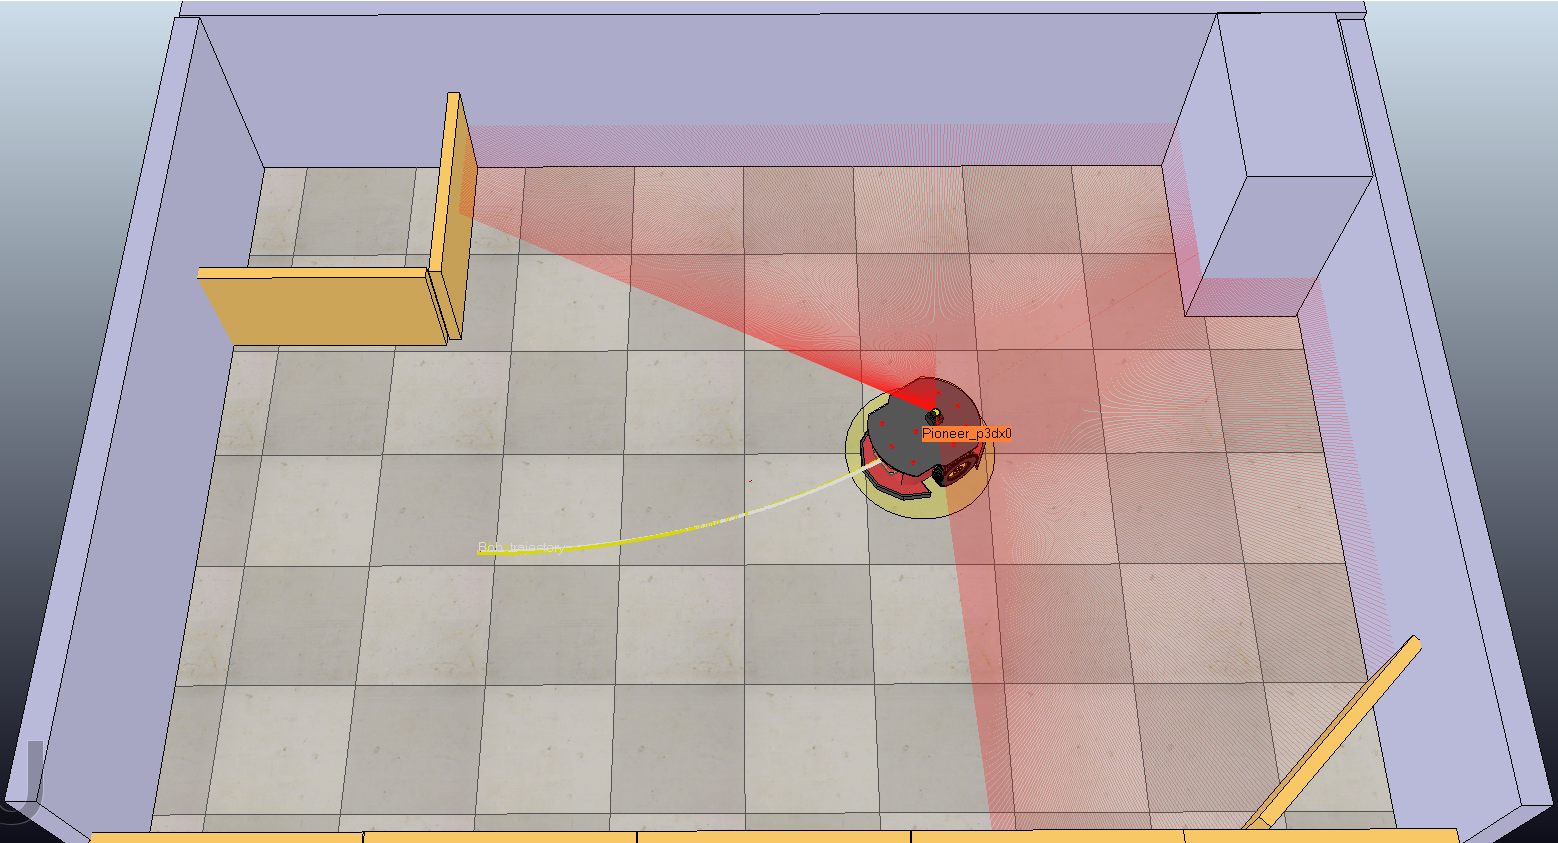
\includegraphics[width=0.9\linewidth]{img/vrep}
	\caption{Estado final do robô na simulação.}
	\label{fig:vrep}
\end{figure}

A implementação da função de localização incremental utilizando filtro de Kalman estendido é dada abaixo:

\begin{lstlisting}[language=Octave]
function [x_posterori, P_posterori] = incrementalLocalization(x, P, u, S, M, params, k, g, l)
% [x_posterori, P_posterori] = incrementalLocalization(x, P, u, S, R, M,
% k, l, g) returns the a posterori estimate of the state and its covariance,
% given the previous state estimate, control inputs, laser measurements and
% the map

C_TR = diag([repmat(0.1^2, 1, size(S, 2)) repmat(0.1^2, 1, size(S, 2))]);
[z, R, ans] = extractLinesPolar(S(1,:), S(2,:), C_TR, params);


%STARTRM
figure(2), cla, hold on;

%compute z_prior
z_prior = zeros(size(M));

for j = 1:size(M, 2)
[z_prior(:,j) H] = measurementFunction(x, M(:,j));
end

plot(z(1,:), z(2,:),'bo');
plot(z_prior(1,:), z_prior(2,:),'rx');
xlabel('angle [rad]'); ylabel('distance [m]')
legend('measurement','prior')
drawnow

% estimate robot pose
[x_posterori, P_posterori] = filterStep(x, P, u, z, R, M, k, g, l); %hint: you just coded this function

%ENDRM
\end{lstlisting}

